\documentclass{beamer}

\usepackage[utf8]{inputenc}
\usepackage[T1]{fontenc}
\usepackage[polish]{babel}
\usepackage{graphicx}
\usetheme[compress]{Berlin}
\usecolortheme{seagull}

\title{Boże Królestwo na Polskiej Ziemi: Wpływ Chrześcijaństwa na Dzieje Polski}
\author{Michał Kraus}
\date{\today}

\begin{document}

% Strona tytułowa
\begin{frame}
    \titlepage
\end{frame}

% Slajd o autorze
\begin{frame}
    \frametitle{Kilka słów o autorze}
    
        Student Politechniki Wrocławskiej.
        Zajmuje się programowaniem i zarządzaniem systemami.
\end{frame}

% Plan prezentacji
\begin{frame}
    \frametitle{Plan prezentacji}
    \begin{itemize}
        \item Cel prezentacji.
        \item Narodziny Polski i ich znaczenie.
        \item Rozwój chrześcijaństwa w Polsce.
        \item Dziedzictwo kulturowe i artystyczne Kościoła.
        \item Chrystus królem Polski i ważne wydarzenia historyczne.
        \item Podsumowanie.
    \end{itemize}
\end{frame}

% Wstęp
\begin{frame}
    \frametitle{Wstęp}
    Celem niniejszej pracy jest przedstawienie wpływu Kościoła rzymskokatolickiego na rozwój i kształtowanie się polskiej tożsamości 
    narodowej oraz kulturowej. Analizując ten wpływ, skupię się na znaczeniu religii katolickiej w kontekście historycznym, cywilizacyjnym i społecznym. 
    Zawarte w pracy rozważania obejmą m.in. rolę Kościoła w tworzeniu fundamentów państwowości polskiej, jego wpływ na kulturę, edukację oraz na kształtowanie 
    wartości narodowych.
\end{frame}

% Chrzest jako narodziny Polski
\begin{frame}
    \frametitle{Chrzest jako narodziny Polski}
    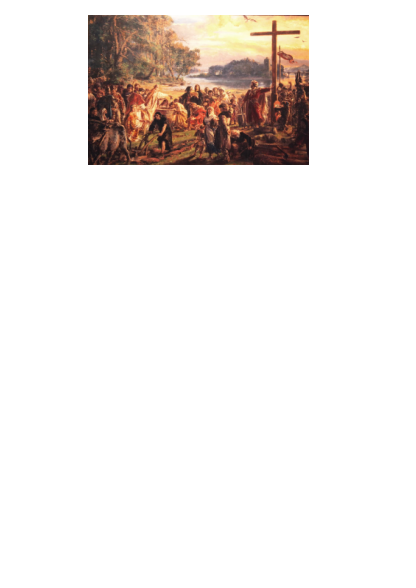
\includegraphics{grafika1.png}
    \begin{itemize}
        \item Symboliczna data: rok 966, chrzest Mieszka I.
        \item Fundament chrześcijańskiej tożsamości Polski.
        \item Znaczenie polityczne: zbliżenie do chrześcijańskiej Europy i sojusze.
    \end{itemize}
\end{frame}

% Rozwój chrześcijaństwa
\begin{frame}
    \frametitle{Rozwój chrześcijaństwa w Polsce: „Bóg, Honor, Ojczyzna”}
    \begin{itemize}
        \item Powstawanie kościołów i katedr.
        \item Wpływ na kulturę i tradycję.
        \item Hasło „Bóg, Honor, Ojczyzna” jako wyraz polskich wartości.
    \end{itemize}
\end{frame}

% Sakralna architektura
\begin{frame}
    \frametitle{Dziedzictwo kulturowe: Sakralna architektura}
    \begin{itemize}
        \item Katedra Wawelska: symbol polskiej państwowości.
        \item Kościół Mariacki: perła gotyckiej architektury.
    \end{itemize}
\end{frame}

% Literatura polska inspirowana wiarą
\begin{frame}
    \frametitle{Literatura polska inspirowana wiarą}
    \begin{itemize}
        \item „Bogurodzica” – najstarsza polska pieśń religijna.
        \item Jan Kochanowski – refleksje nad wiarą w „Trenach”.
        \item Henryk Sienkiewicz – „Quo Vadis” jako odwołanie do chrześcijaństwa.
    \end{itemize}
\end{frame}

% Chrystus królem Polski
\begin{frame}
    \frametitle{Chrystus królem Polski}
    \begin{itemize}
        \item Śluby Lwowskie (1656) – oddanie Polski pod opiekę Maryi.
        \item Cud nad Wisłą (1920) – uznanie zwycięstwa za interwencję boską.
        \item Poświęcenie Polski Najświętszemu Sercu Jezusowemu.
    \end{itemize}
\end{frame}

% Podsumowanie
\begin{frame}
    \frametitle{Podsumowanie}
    \begin{itemize}
        \item Ukazano wpływ wiary na historię Polski.
        \item Wskazano na dziedzictwo kulturowe inspirowane religią.
        \item Wiarę przedstawiono jako fundament polskiej tożsamości.
    \end{itemize}
\end{frame}

% Bibliografia
\begin{frame}
    \frametitle{Bibliografia}
    \begin{itemize}
        \item Jan Paweł II. Pielgrzymka do Ojczyzny. Kraków: Znak, 1979.
        \item Jezus Chrystus Król Wszechświata - Parafia Sikórz.
        \item Obraz Chrztu Mieszka I – dostęp online.
    \end{itemize}
\end{frame}

\end{document}
